\documentclass[12pt]{article}
\setlength{\columnsep}{1cm}
\usepackage{fullpage}
\usepackage{titlesec}
\usepackage{enumerate}
\usepackage{amsmath}
\usepackage{amsthm}
\usepackage{paralist}
\usepackage{fancyhdr}
\usepackage{graphicx}
\titleformat{\subsubsection}[runin]{}{}{}{}[]
\renewcommand{\labelenumi}{\alph{enumi}.}
\pagestyle{fancyplain}
\setlength{\headsep}{30.4pt}

\lhead{
\includegraphics[scale=0.5]{../public/sharematch.png}}
\rhead{Final Project Report}
\cfoot{\today}

\begin{document}
\section*{Final Project Report}
\begin{itemize}
    \item \textbf{Ian Dimayuga (icd3)}
    \item \textbf{Tom Dooner (ted27)}
    \item \textbf{Brian Stack (bis12)}
\end{itemize}
\subsection*{ER Diagram}
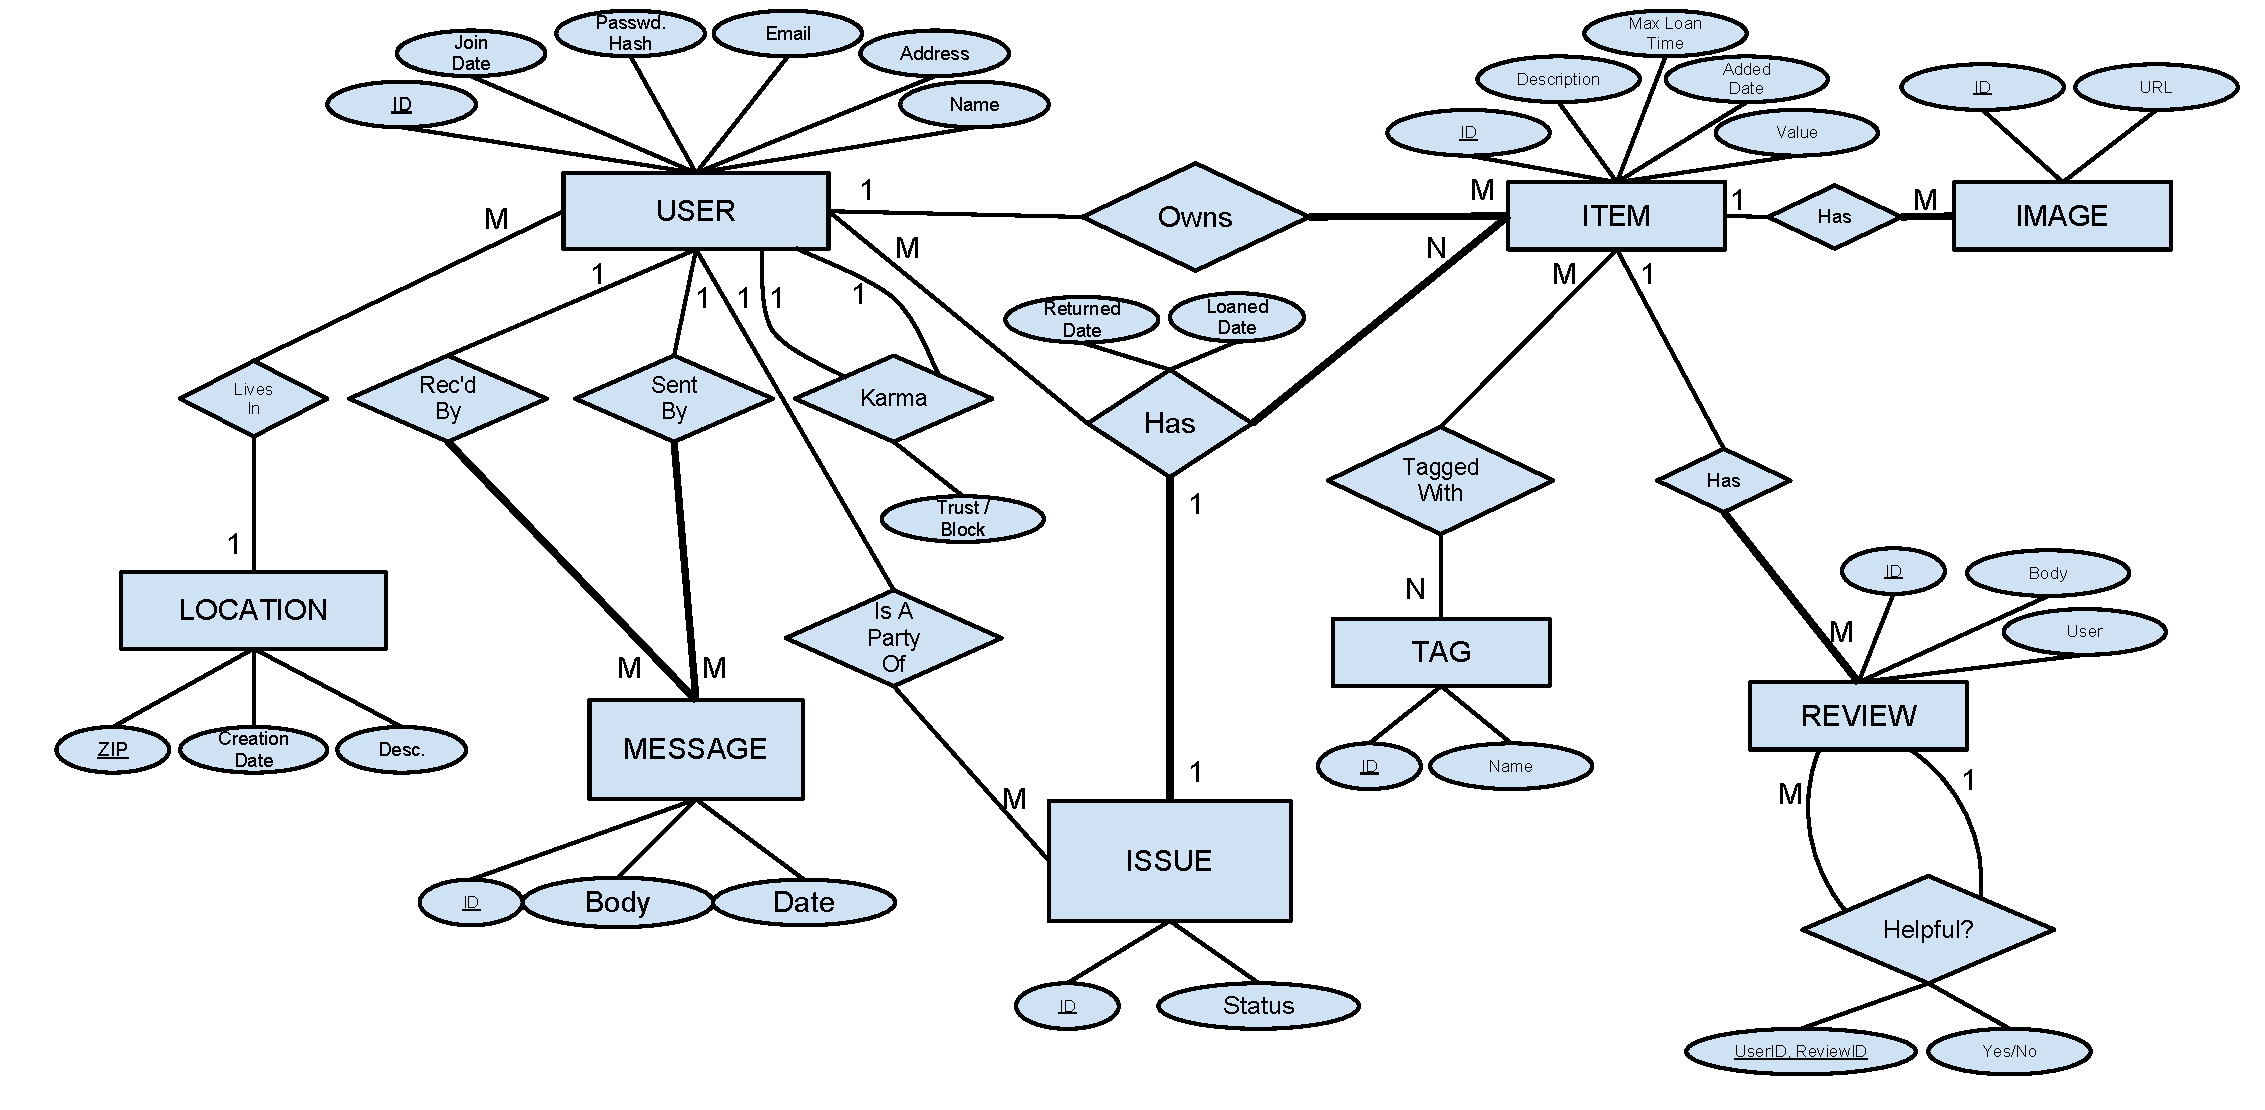
\includegraphics[scale=0.5]{EECS341ProjectERDiagram.pdf}

\subsection*{Relational Diagram}
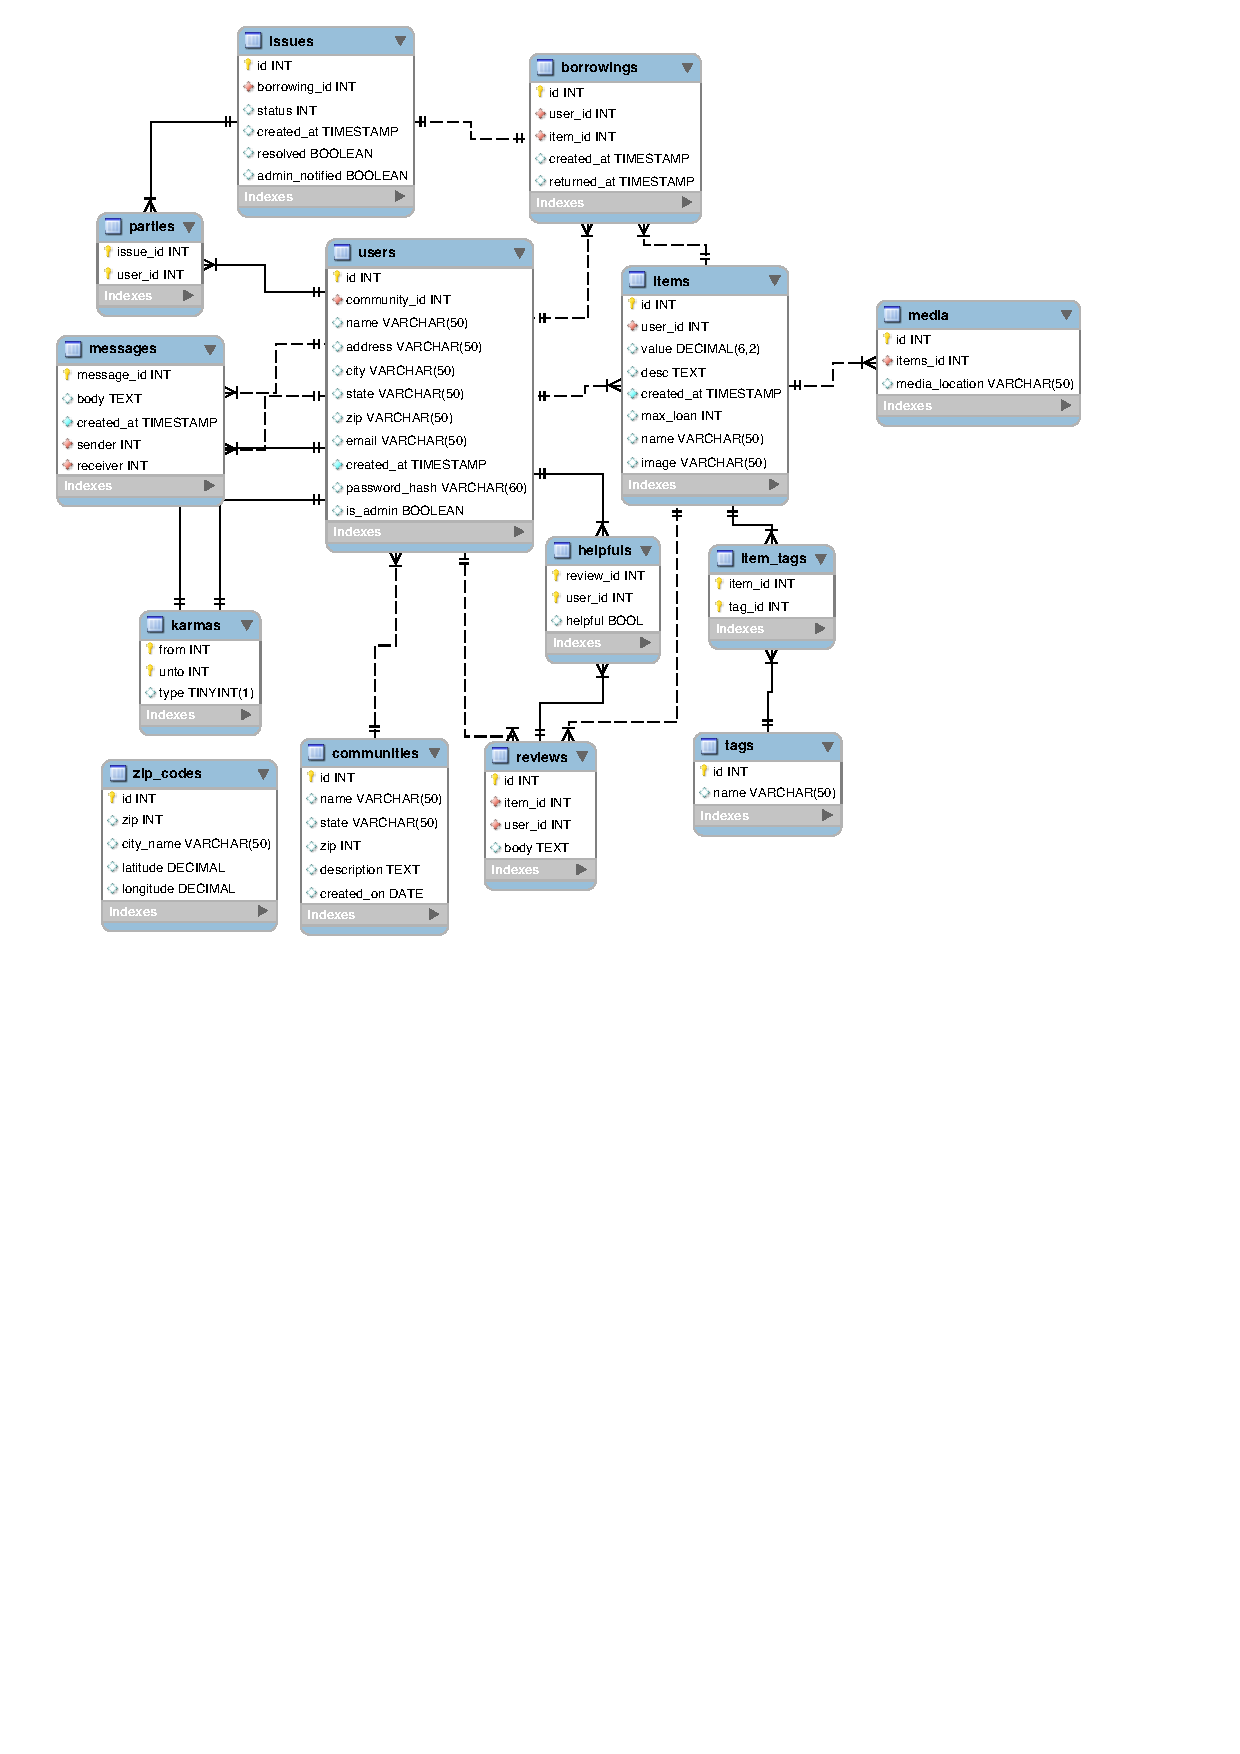
\includegraphics[trim=0in 4in 0in 0in,clip=true,width=8in]{EECS341Relational.pdf}

\subsection*{Commands To Create Database}
\begin{verbatim}
CREATE TABLE "borrowings" ("borrow_id" INTEGER NOT NULL PRIMARY KEY 
  AUTOINCREMENT, "borrow_at" TIMESTAMP, "user_id" INTEGER, "item_id" INTEGER);

CREATE TABLE "helpfuls" ("review_id" INTEGER NOT NULL, "user_id" INTEGER 
  NOT NULL, "helpful" BOOLEAN, PRIMARY KEY("review_id", "user_id"));

CREATE TABLE "issues" ("issue_id" INTEGER NOT NULL PRIMARY KEY 
  AUTOINCREMENT, "created_at" TIMESTAMP);

CREATE TABLE "items" ("id" INTEGER NOT NULL PRIMARY KEY AUTOINCREMENT, 
   "value" DECIMAL(6, 2), "created_at" TIMESTAMP, "max_loan" INTEGER, 
   "user_id" INTEGER);

CREATE TABLE "karmas" ("from" INTEGER NOT NULL, "unto" INTEGER NOT NULL, 
    "type" BOOLEAN, PRIMARY KEY("from", "unto"));

CREATE TABLE "locations" ("zip_code" INTEGER NOT NULL, "description" TEXT, 
    "created_on" DATE, PRIMARY KEY("zip_code"));

CREATE TABLE "media" ("media_id" INTEGER NOT NULL PRIMARY KEY AUTOINCREMENT, 
    "item_id" INTEGER, "media_location" VARCHAR(50));

CREATE TABLE "messages" ("message_id" INTEGER NOT NULL PRIMARY KEY 
    AUTOINCREMENT, "body" TEXT, "created_at" TIMESTAMP, "sender" INTEGER, 
    "reciever" INTEGER);

CREATE TABLE "parties" ("issue_id" INTEGER NOT NULL, "user_id" INTEGER 
    NOT NULL, PRIMARY KEY("issue_id", "user_id"));

CREATE TABLE "reviews" ("item_id" INTEGER NOT NULL, "user_id" INTEGER NOT 
    NULL, "body" TEXT, PRIMARY KEY("item_id", "user_id"));

CREATE TABLE "taggings" ("item_id" INTEGER NOT NULL, "tag_id" INTEGER NOT 
    NULL, PRIMARY KEY("item_id", "tag_id"));

CREATE TABLE "tags" ("tag_id" INTEGER NOT NULL PRIMARY KEY AUTOINCREMENT, 
    "name" VARCHAR(50));

CREATE TABLE "users" ("id" INTEGER NOT NULL PRIMARY KEY AUTOINCREMENT, 
    "name" VARCHAR(50), "address" VARCHAR(50), "location_id" INTEGER, 
    "email" VARCHAR(50), "joined_at" TIMESTAMP, "password" INTEGER);
\end{verbatim}

\section*{Project Report 3}
\subsection*{Actual Database CREATE TABLE Commands}
\begin{verbatim}
~ (0.000059) SELECT sqlite_version(*)
~ (0.094862) DROP TABLE IF EXISTS "users"
~ (0.000048) PRAGMA table_info("users")
~ (0.083899) CREATE TABLE "users" ("id" INTEGER NOT NULL PRIMARY KEY 
    AUTOINCREMENT, "name" VARCHAR(50), "address" VARCHAR(50), "location_id" 
    INTEGER, "email" VARCHAR(50), "joined_at" TIMESTAMP, "password" VARCHAR(50))
~ (0.077341) DROP TABLE IF EXISTS "items"
~ (0.000044) PRAGMA table_info("items")
~ (0.084186) CREATE TABLE "items" ("id" INTEGER NOT NULL PRIMARY KEY 
    AUTOINCREMENT, "value" DECIMAL(6, 2), "created_at" TIMESTAMP, "max_loan" 
    INTEGER, "user_id" INTEGER)
~ (0.077268) DROP TABLE IF EXISTS "borrowings"
~ (0.000051) PRAGMA table_info("borrowings")
~ (0.092402) CREATE TABLE "borrowings" ("borrow_id" INTEGER NOT NULL 
    PRIMARY KEY AUTOINCREMENT, "borrow_at" TIMESTAMP, "user_id" INTEGER, 
    "item_id" INTEGER)
~ (0.077277) DROP TABLE IF EXISTS "issues"
~ (0.000052) PRAGMA table_info("issues")
~ (0.084420) CREATE TABLE "issues" ("issue_id" INTEGER NOT NULL PRIMARY KEY 
    AUTOINCREMENT, "created_at" TIMESTAMP)
~ (0.085705) DROP TABLE IF EXISTS "parties"
~ (0.000042) PRAGMA table_info("parties")
~ (0.092652) CREATE TABLE "parties" ("issue_id" INTEGER NOT NULL, "user_id" 
    INTEGER NOT NULL, PRIMARY KEY("issue_id", "user_id"))
~ (0.069049) DROP TABLE IF EXISTS "messages"
~ (0.000038) PRAGMA table_info("messages")
~ (0.076223) CREATE TABLE "messages" ("message_id" INTEGER NOT NULL 
    PRIMARY KEY AUTOINCREMENT, "body" TEXT, "created_at" TIMESTAMP, "sender" 
    INTEGER, "reciever" INTEGER)
~ (0.085388) DROP TABLE IF EXISTS "karmas"
~ (0.000041) PRAGMA table_info("karmas")
~ (0.089046) CREATE TABLE "karmas" ("from" INTEGER NOT NULL, "unto" 
    INTEGER NOT NULL, "type" BOOLEAN, PRIMARY KEY("from", "unto"))
~ (0.072760) DROP TABLE IF EXISTS "tags"
~ (0.000041) PRAGMA table_info("tags")
~ (0.078664) CREATE TABLE "tags" ("tag_id" INTEGER NOT NULL PRIMARY KEY i
    AUTOINCREMENT, "name" VARCHAR(50))
~ (0.124553) DROP TABLE IF EXISTS "taggings"
~ (0.000039) PRAGMA table_info("taggings")
~ (0.088938) CREATE TABLE "taggings" ("item_id" INTEGER NOT NULL, 
    "tag_id" INTEGER NOT NULL, PRIMARY KEY("item_id", "tag_id"))
~ (0.072803) DROP TABLE IF EXISTS "media"
~ (0.000049) PRAGMA table_info("media")
~ (0.080807) CREATE TABLE "media" ("media_id" INTEGER NOT NULL PRIMARY KEY 
    AUTOINCREMENT, "item_id" INTEGER, "media_location" VARCHAR(50))
~ (0.072807) DROP TABLE IF EXISTS "locations"
~ (0.000041) PRAGMA table_info("locations")
~ (0.089033) CREATE TABLE "locations" ("zip_code" INTEGER NOT NULL, 
    "description" TEXT, "created_on" DATE, PRIMARY KEY("zip_code"))
~ (0.072825) DROP TABLE IF EXISTS "reviews"
~ (0.000040) PRAGMA table_info("reviews")
~ (0.079151) CREATE TABLE "reviews" ("item_id" INTEGER NOT NULL, "user_id" 
    INTEGER NOT NULL, "body" TEXT, PRIMARY KEY("item_id", "user_id"))
~ (0.069770) DROP TABLE IF EXISTS "helpfuls"
~ (0.000032) PRAGMA table_info("helpfuls")
~ (0.072982) CREATE TABLE "helpfuls" ("review_id" INTEGER NOT NULL, 
    "user_id" INTEGER NOT NULL, "helpful" BOOLEAN, PRIMARY KEY("review_id", 
    "user_id"))
\end{verbatim}
\end{document}
